\documentclass[11pt]{article}
\usepackage[margin=1.2in,footskip=0.25in]{geometry}
\usepackage{amsmath}
\usepackage{algorithmicx}
\usepackage{algpseudocode}
\usepackage{graphicx}
\usepackage{subfigure}
\usepackage{float}
\usepackage[authoryear]{natbib}

%Gummi|065|=)
\title{\textbf{Advanced Algorithms - Minimum tardiness scheduling}}
\author{Lu Dai (4506677)\\
		Yuxuan Kang (4504410)\\}
\date{16 Nov 2016}
\begin{document}

\maketitle

\makeatletter
\def\BState{\State\hskip-\ALG@thistlm}
\makeatother
\section{Problem description}
Given one machine to process $n$ jobs $j_1, j_2,...,j_n$. Each job $j_i$ has a processing time $p_i$ and a due time $d_i$, the tardiness of a job is to describe how much time a job is late from its due time, thus defined as:
$$t_i=max\{0,c_i-d_i\}$$
where $c_i$ is the completion time of the job $j_i$.\\
The problem of minimizing tardiness scheduling is to find a schedule that minimize the total tardiness. The total tardiness is defined as:
$$total\ \ tardiness=\sum_{i=1}^n t_i$$ 

In this report, there are two methods implemented:
\begin{enumerate}
\item an exact algorithm, which can find an optimal solution to this problem.
\item an FPTAS, which produces a solution that is within a factor $1+\epsilon$ of being optimal.	
\end{enumerate}

After the implementation of these two methods, comparisons between these two algorithms together with greedy algorithm and best-fit algorithm are carried out. Finally there is a discussion about the results and runtime of these four algorithms.

\section{Exact algorithm}\label{Exact algorithm}
The exact algorithm is based on a dynamic programming method from the article by Lawler(1977). A tree structure is created to split the problem into smaller problems. By solving the smaller problems, the complete problem will be solved eventually.

In this dynamic programming approach, all the jobs are firstly sorted in non-decreasing due time order. The job k with maximum processing time $p_k$ is found. Given an integer $\delta$ ($\delta \in [0,n-k]$), the sequence is going to be reformed to three parts: 

\begin{description}
\item[$(i)$]First part: $j_1,j_2,...,j_{k-1},j_{k+1},...,j_{k+\delta }$
\item[$(ii)$]Second part: $j_k$
\item[$(iii)$]Third part: $j_{k+\delta +1},j_{k+\delta +2},...,j_n$
\end{description}

The first and the third parts can be regarded as subsets of the sequence. The whole schedule is optimal if and only if these two sub-schedules are optimal. It implies a recursive way of solving this problem. Each subset is the same problem but with smaller size. The subset S, with an interval $i,i+1,...j$ and with all processing time being less than $p_k$, can be denoted as:
$$S(i,j,k)=\{j'|i\leq j'\leq j, p_{j^{'}}<p_k\}$$
Thus the total tardiness of a subset $T(S(i,j,k),t)$ with a start time $t$ will be:
$$T(S(i,j,k),t)=min_{\delta} \{ T(S(i,k'+\delta,k'),t)+w_{k'}max(0,C_{k{'}}(\delta)-d_{k'})+T(S(k'+\delta+1,j,k'),C_{k'}(\delta)) \}$$
where $k'$ is such that:$$p_{k'}=max{p_{j'}|j' \in S(i,j,k)},$$
$$C_{k'}(\delta) =t+\sum_{i\leq j' \leq k'+\delta}p_{j'}$$ 

In the paper by Lawler(1977), the run time of this algorithm was also analyzed. A upper bound on the worst-case running time is established. There are no more than $O(n^3)$ subsets $S(i,j,k)$. Besides, there are no more than $P=\sum p_j \leq np_{max}$ possible values of $t$. Based on this observation, the number of equations need to be solved is bounded by $O(n^4p_{max})$. For each equation, $O(n)$ running time is needed for minimizing tardiness over at most $n$ alternatives. Thus the overall run time is bounded by $O(n^5p_{max})$.
\subsection{Refinements of the algorithm}

The runtime can be significantly reduced by two means:
\begin{enumerate}
\item Restrict the options of $\delta$. For each $\delta$, the program will go to a separate recursion. Thus, the number of the choices of $\delta$ will have a huge influence on the number of trees generated. By restricting the options of $\delta$, the algorithm will be much improved. 
\item Store optimal solution of a subset. The same subset is not necesssary to calculate repeatly, thus if a subuset has the same jobs and the same start time as some subset already stored, the schedule of this subset can be retrieved directly.

The restriction of $\delta$ is based on the fact that if job $k$ has due date $d_k$, then there exists an optimal sequence in which the completion time of job $k$ is at least as large as $d_{k'}$, where $d_{k'}=t+\sum _{j\in S'}p_j$ and $S'=\{ j| d_j \leq d_k, j\in S \}$

In the next section, the pseudo-code will show how the refinements are implemented. Function \textbf{\textit{getDelta()}} restrict the selections of $\delta$, and hashmap \textbf{\textit{cache}} stores the optimal schedules which have been processed. There is a chain structure $Schedule$ defined. It consists of three parts, the first parameter is $Schedule$ structure which stores the schedule before this job, the second parameter and the third parameter are the processing time and the due time of this job respectively.
\end{enumerate}

\subsection{Pseudo-code of exact algorithm}
\begin{algorithmic}
\State Structure $Schedule$ \{ $Schedule,\ \ processing\ \ time, due\ \ time $ \}
\State Sort all jobs in non-decreasing order of due times
\Function{GetSchedule}{$schedule$, $Jobs$, $t_{start}$}
\If {$Jobs$ is $\emptyset$ }
    \State $return\ \ schedule$
\EndIf
\If {$cache$ contains ($Schedule(t_{start}$,$Jobs$))}
    \State $return$ $cache.getSchedule(t_{start},Jobs)$
\EndIf

\State $k \gets$ index of job with the largest processing time
\State $optimalSchedule\gets null$
\State $\{ \delta_{1},\delta_{2}..., \delta_{m} \} \gets getDelta(Jobs, k, t_{start})$
 \For {each $\delta\ \ in\ \ \{ \delta_{1},\delta_{2}..., \delta_{m} \}$}
\State $front\_Jobs \gets \{ j_1,j_2,...,j_{k-1},j_{k+1},...,j_{k+\delta }\}$
\State $front\_Schedule \gets getSchedule(schedule,front\_Jobs,t_{start})$ 
\State $ScheduleK= Schedule(front\_Schedule,p_k,d_k)$
\State $back\_Jobs \gets \{j_{k+\delta+1},...,j_{n}\}$
\State $back\_Schedule \gets getSchedule(ScheduleK,back\_Jobs,C_k(\delta))$
 \If {$optimalSchedule.tardiness > back\_Schedule.tardiness$}
    \State $optimalSchedule=back\_Schedule$
\EndIf
    
\EndFor
\State $return$ $optimalSchedule$


 
\EndFunction\\
\Function{GetDelta}{$Jobs$, $k$, $t_{start}$}
\State $n\gets number of jobs$
\While{true}
\State $S' \gets \{j \in Jobs|d_j\leq d_k\}$
\State $d_{k'}\gets t_{start}+\sum _{j\in S'}p_j$
 \If {$d_k<d_{k'}$}
    \State $d_k\gets d_{k'}$
\EndIf
\State $\delta \gets max_j{S'}-k$
\State $S_{\delta}\gets add \ \ \delta$
\State $S''=\{j\in Jobs|d_j>d_k\}$
\State $d_{j'}\gets min_{j\in S''}d_j$
 \If {$j'\geq n$}
    \State $return \ \ S_{\delta}$
\EndIf
\State $d_{k'}\gets d_{j'}$
\EndWhile
\EndFunction
\end{algorithmic}
\section{Approximation algorithm}
An approximation algorithm for this problem was also carried out by Lawler(1982). In this paper, a fully polynomial approximation scheme for this problem is implemented by scaling method. Denote the tardiness of job $j$ as $T_j=max\{ 0,C_j-d_j\}$, all the jobs are firstly sequenced in nondecreasing order of due dates. Then the maximum tardiness of the jobs $T_{max}=max\{ T_j\}$ is found. Given a parameter $\epsilon$, the scaling coeffcient $K$ will be: 
$$K=\frac{2\epsilon}{n(n+1)}T_{max}$$

All the processing times can be rescaled by this coeffienct $K$, thus the rescaled processing time of job $j$ will be:
$$q_j=\Bigl\lfloor \frac{p_j}{K} \Bigr\rfloor $$
And the due date also need to be rescaled as:
$$b_j=\frac{d_j}{K}$$

Apply the same exact algorithm in section \ref{Exact algorithm} on rescaled processing times and due times, an approximate solution $T_A$ will be obtained, which satisfies:
$$T_A \leq (1+\epsilon) T^*$$

Lawler(1982) also presented a run time analysis on the approximation algorithm. The run time is upper bounded by $K$ value and $T_{max}$: $O(n^5T_{max}/K)$. Based on the relation between $K$ and $T_{max}$, the run time can be rewritten into $O(n^7/\epsilon)$. Thus the run time is polynomial in $n$ and bounded by $\epsilon$, proving it as a FPTAS.
\subsection{Pseudo-code of approximation algorithm}

\begin{algorithmic}
\State Sort all jobs in non-decreasing order of due times
\State $t\gets 0$
\State $n\gets number of Jobs$
\State $T_{max}\gets -1$
\For {each $job_j$}  // find the maximum tardiness of the jobs
    \State $t \gets t+p_i$
    \State $T_j\gets max\{ 0,t-d_j\}$
    \If {$T_j >T_{max}$}
    \State $T_{max}\gets T_j$
    \EndIf
\EndFor
\State $K\gets \frac{2\epsilon}{n(n+1)}T_{max}$
\For {each $job_i$} // rescale processing times and due times
    \State $q_i\gets \Bigl\lfloor \frac{p_i}{K} \Bigr\rfloor$
    \State $b_i\gets \frac{d_j}{K}$
\EndFor
\State $schedule \gets$ $ExactAlgorithm(q_i,b_i)$ //run exact algorithm on rescaled $p$ and $d$
\State $T \gets 0$
\State $t\gets 0$
\For {each $job_i$ in $schedule$} //use original $p$ and $d$ to calculate total tardiness
	\State $t \gets t+p_i$
    \State $T \gets$ $T+max\{ 0, t-d_i\}$
\EndFor
\State $return\ \ T$
\end{algorithmic}
\section {Result}
In this chapter, the two implemented algorithms will be compared. They are tested on 500 instances, with the smallest instance of 5 jobs and the largest instance of 100 jobs. The correctness of each algorithm will be checked and the run time of them will be compared. According to the characteristics of exact and approximation algorithms, it is known that exact algorithm will cost much more time to find an optimal solution for the problem while approximation algorithm will cost much less time with the price of non-optimal solutions.\\
The following figure shows the result from three algorithms (greedy, exact and approximation algorithm). It can be easily observed that the tardiness grows quckily with the increasement of instance sizes. In addition, approximation algorithms with smaller epsilon values holds better results than higher epsilons, which are closer to optimal results.
\begin{figure}[H]
  \centering
    \label{fig:runtime} %% label for first subfigure
    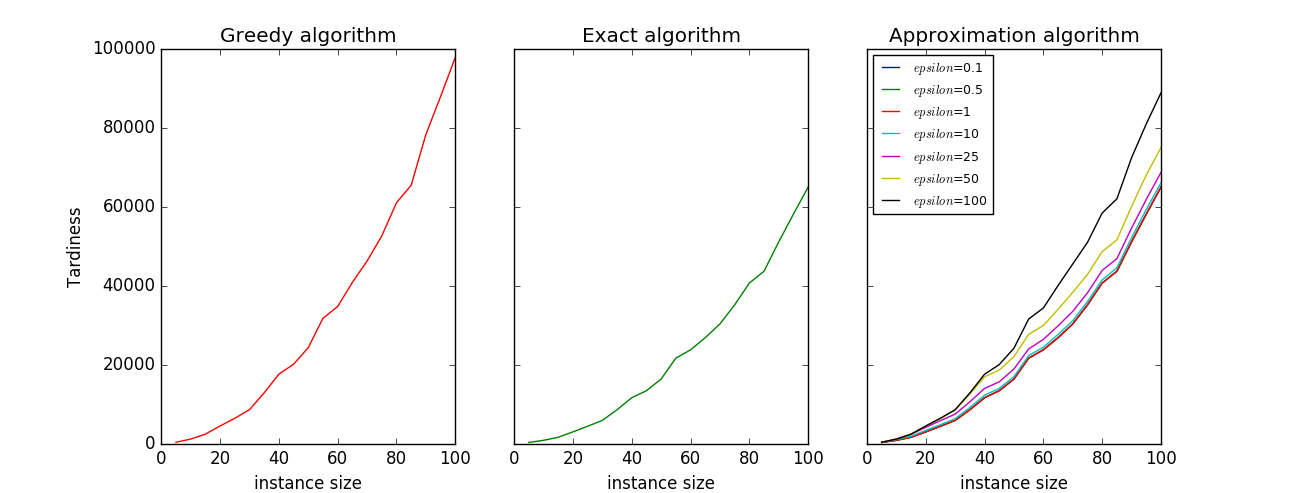
\includegraphics[width=1.1\textwidth]{three_alg.png}
	\caption{The tardiness of the three algorithms}
\end{figure}
\subsection{Run time of exact and approximation algorithm}
\begin{figure}[H]
  \centering
    \label{fig:runtime} %% label for first subfigure
    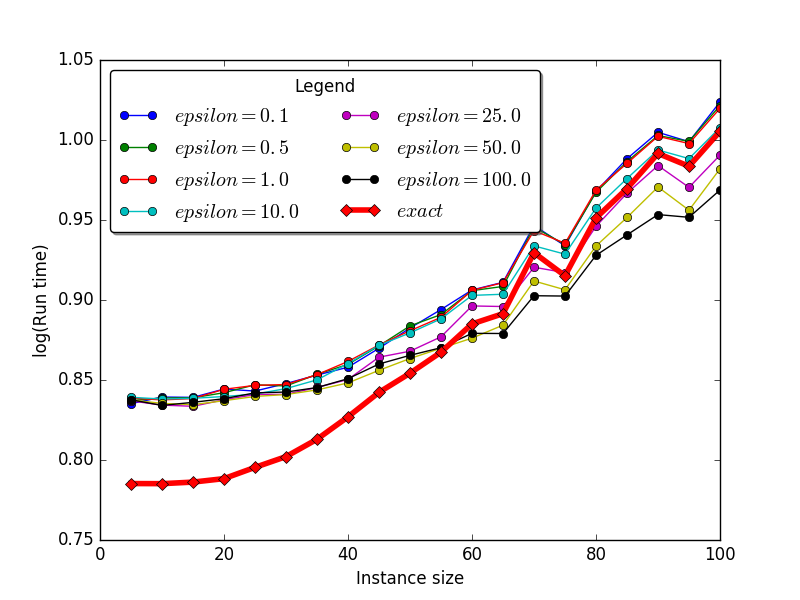
\includegraphics[width=1\textwidth]{runtime.png}
\caption{Run time of exact algorithm and approximation algorithm}
\end{figure}
The above figure shows the run time of exact algorithm and approximation algorithm. X-axis denotes size of instances ranging from 5 to 100 jobs while y-axis denotes the logarithm of the run time. The run time is calculated by averaging the run time of instances with different $rdd$ and $tf$ but same instance size. The thick red line represents the run time of exact algorithm, and other lines represent run time of approximation algorithms with different epsilon value.\\
There are certain rules contained in the figure:
\begin{enumerate}
\item All the run time follow a growing trend with repect to the incresement of instance size.
\item Aprroximation algorithms with lower epsilons tend to cost more time than higher ones.
\item Exact algorithm runs much fast than approximation in small instance sizes. However, after some certain point of instance size(around 50), some approximation algorithms with proper epsilon values grab better performance in runtime.
\end{enumerate}
In the experiment, when $\epsilon$ is 0.1, 0.5 or 1, the approximation algorithm seems to cost more time no matter of the size of the instance. It is probably because the instance is not rescaled that much and approximation algorithm also calls the exact algorithm. Thus the approximation algorithm actually doesn't save time in these situations. Instead, it does some extra rescaling work, so it will cost more time when epsilon is small. Considering Figure 1 and 2 together, which contains the information of the balanced points of result and runtime.
\subsection{Tardiness of different RDD and TF}
\begin{figure}[H]
\hspace*{-1cm} 
  \centering%% label for first subfigure
    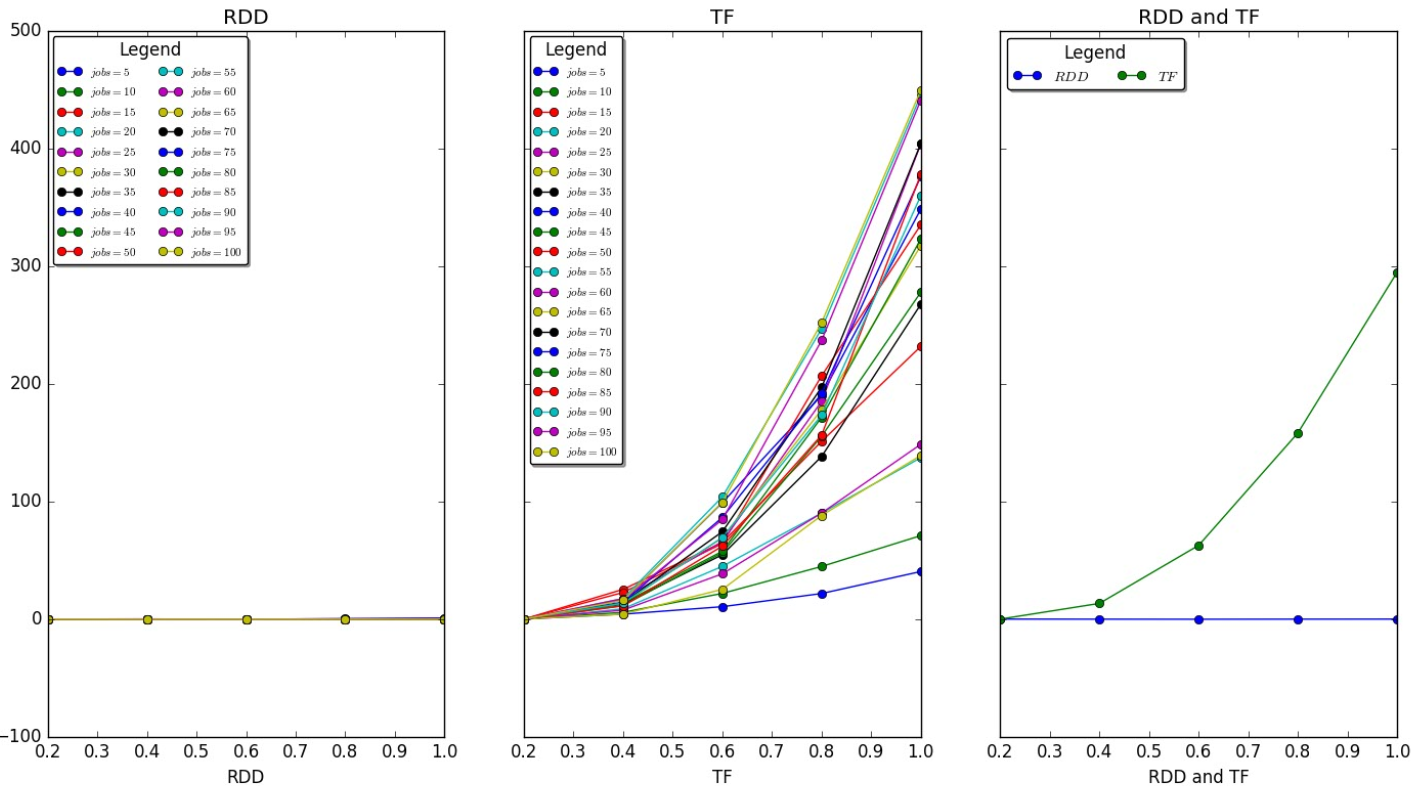
\includegraphics[width=1.2\textwidth]{RDD_TF_tardiness.png}
	\caption{Tardiness-RDD and Tardiness-TF}
	\label{fig:RDD_TF_t}
\end{figure}
Figure \ref{fig:RDD_TF_t} show how RDD and TF influence on the tardiness w.r.t instance size, and the third sub-figure is the average of all the instances. The x-axis is the value of RDD/TF value, and the y-axis is the normalized value of the increase or decrease compared to RDD/TF =0.2. It is calculated as follows:
$$ y= \frac{tardiness(x)-tardiness(0.2)}{tardiness(0.2)}$$
It is clear to see for all the instances, RDD does not have much influence on the tardiness value. The tardiness remains almost the same for all the instances. However, it is obvious that TF value has much influence on the tardiness. With the increase of TF value, the tardiness for all the instances increases largely. Figure \ref{fig:RDD_TF_t} clearly compares the influence power between RDD and TF. RDD and TF determine the distribution of the due times where RDD determines the range of the due time and TF determines the average due time value. Larger TF means smaller average due time, which means less jobs will be finished on time, which leads to larger total tardiness.

\subsection{Run time of different RDD and TF}
\begin{figure}[H]
\hspace*{-1cm} 
    \label{fig:runtime} %% label for first subfigure
    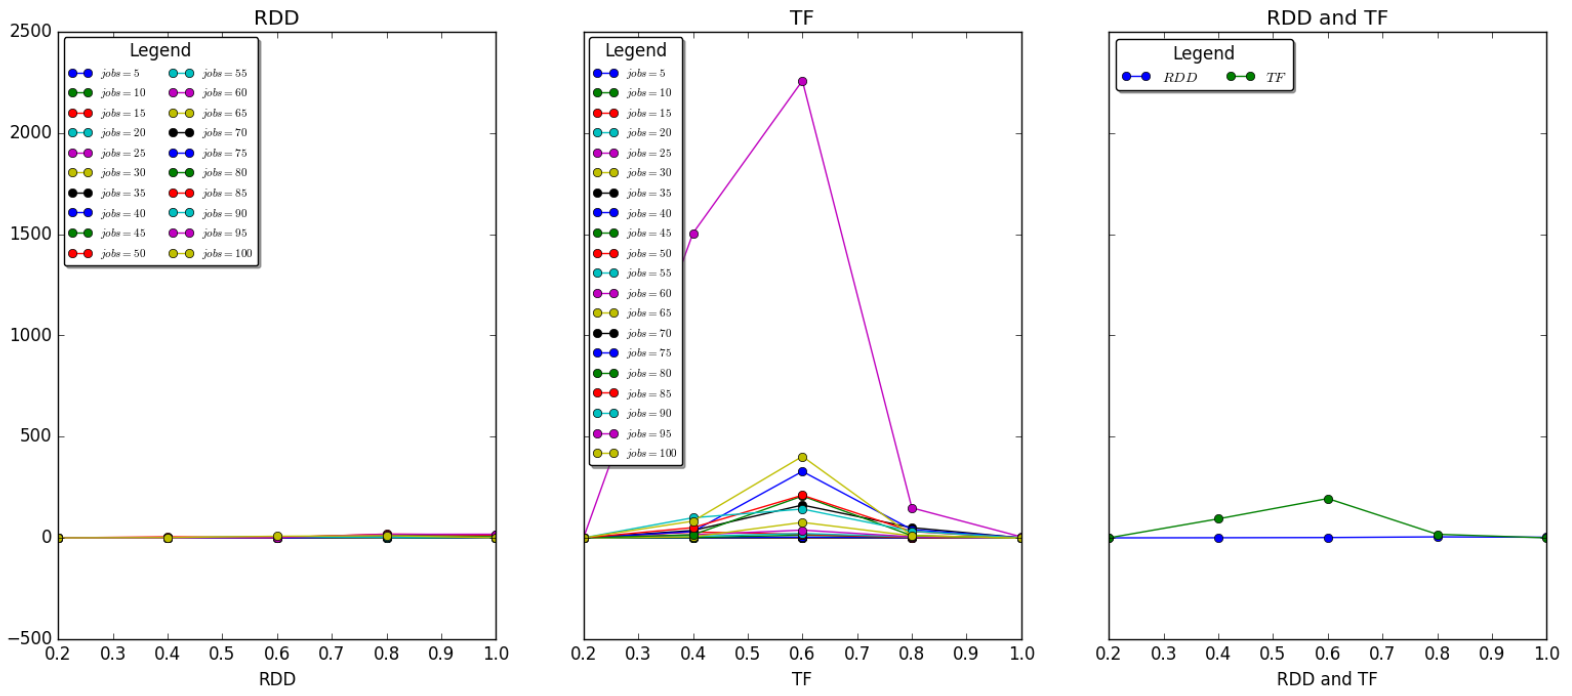
\includegraphics[width=1.2\textwidth]{RDD_TF_runtime.png}
	\caption{Run time-RDD and runtime-TF}
	\label{fig:RDD_TF_runtime}
\end{figure}
Similar to the analysis on tardiness with different RDD and TF, an experiment is carried out for the run time and different RDD and TF. Y-axis is the normalized value of the increase or decrease compared to RDD/TF =0.2:
$$ y= \frac{runtime(x)-runtime(0.2)}{runtime(0.2)}$$
It is observed that RDD still has little influence on the runtime while TF is in a more tricky situation. It is worth noting that when TF=0.6, the runtimes reach their peak, holding almost for all instance sizes.  As literature shows, the most complicated instances are generated by TF=0.6, which is proved in our experiments. The reason behind this heavily relies on the distribution of  job due times.
\subsection{Performance ratio of approximation algorithm}
\begin{figure}[H]
\hspace*{-1cm} 
    \label{fig:runtime} %% label for first subfigure
    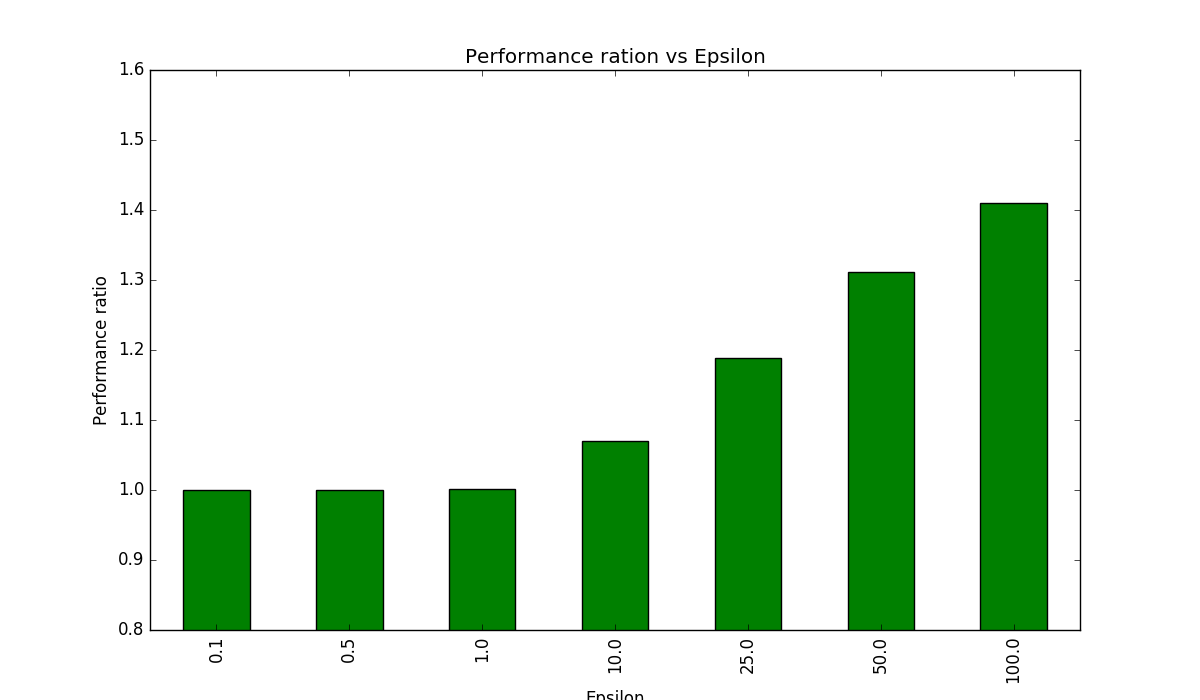
\includegraphics[width=1.2\textwidth]{performance_ratio.png}
	\caption{Performance ratio of approximation algorithm}
\end{figure}
The performance ratio of the approximation algorithm is shown in the above figure. The performance ratio is calculated by averaging the performance ratio of each instance. When $\epsilon=$ 0.1, 0.5, 1.0, the approximation algorithm can reach optimal solutions, however it costs at least as much time as exact algorithm as discussed in previous sections.  When $\epsilon$ is greater than 10, the approximation begins to get non-optimal solution bounded by the factor $\epsilon$ where the worst performance happen on  $\epsilon$= 100. However, the growing trend of performance ratio is getting smaller.
\subsection{Practical Use}For many NP problems, it is practical to decide whether to use exact algorithm to reach  optimal solutions or use approximation algorithm to get a near optimal solution with much less time. According to the experiments in previous subsections, exact algorithm performs very well in this case. It cost similar time even less time than approximation algorithm when $\epsilon$ is small to reach the optimal solution. Because the exact algorithm Lawler proposed has been refined with several approaches, the run time is shortened to be acceptable and it gains optimal solution at the same time. Therefore, in practice, this exact algorithm is more feasible.
\nocite{*}
\bibliographystyle{plainnat}
\bibliography{Programming.bib}

\end{document}
